\chapter{Global Sensitivity Analysis}

\new{
Global sensitivity analysis (GSA) involves a quantitative assessment of variability in the
model output or quantity of interest (QoI) due to uncertain model parameters. Variance based
approaches relying on pseudo-random sampling of prior distributions of the parameters
have been used effectively~\cite{Cukier:1973, Sobol:1990, Saltelli:2008}. However, it can
be understood that estimating the sensitivity indices (`first order effect' and `total
effect') can
be computationally intensive especially in situations where a complex multiphysics model
is simulated for a considered set of parameter samples. In order to mitigate such computational
costs, alternative strategies involving construction and application of cheap surrogates for the
models have been developed. Examples include polynomial chaos
expansions~\cite{Xiu:2002, Ghanem:2003} which have been used extensively for physics-based
models and admit simple analytical expressions for computing the sensitivity
indices~\cite{Vohra:2014, Vohra:2016}. 
Other examples include
response surfaces based on Kriging, and radial basis functions~\cite{Gutmann:2001}. 

Surrogate models, however, are not the central theme of this chapter. Instead, we focus
our attention on exploiting QUESO to perform a prior based, parametric GSA. As mentioned 
earlier, the analysis helps determine relative contribution to the variance of the QoI and 
thus the relative importance of the stochastic model parameters. Potentially, such an 
analysis could help reduce the dimensionality of an inverse problem. In the following section,
we provide a mathematical framework for the first order effect and total effect sensitivity indices
as well as a brief survey of existing estimators for these indices. In section~\ref{sec:app},
we provide an algorithm based on~\cite{Saltelli:2010}
for using QUESO to perform a prior-based parametric GSA and
further demonstrate its implementation using a simple exercise involving sensitivity analysis
of the slope and intercept of a straight line.  
 
}

\section{Sensitivity Indices}

Consider a model, $\mathcal{G}(\bm \theta)$, where $\bm \theta$ denotes a vector of model
parameters. Variance based measures for the first order effect and total effect sensitivity
indices can be computed as discussed below. 

\subsection{First Order Effect}

The first order effect sensitivity index $\mathcal{S}(\theta_{i})$ for a specific model
parameter $(\theta_{i})$ quantifies relative contribution to the variance of the QoI
strictly due to $(\theta_{i})$ and does not consider its interactions with other parameters.
Mathematically, this is expressed as follows:

\be
\mathcal{S}(\theta_{i}) = \frac{\V_{\theta_{i}}(\E_{\bm \theta_{\sim i}}[\mathcal{G}\vert\theta_{i}])}{\V(\mathcal{G})}
\ee

\noindent where $\theta_{i}$ is the $i^{th}$ parameter for which the first order effect index is to be
computed and $\bm \theta_{\sim i}$ denotes a vector of all parameters except $\theta_{i}$. The quantity,
$\E_{\bm \theta_{\sim i}}[\mathcal{G}\vert\theta_{i}]$ denotes the mean estimate of the model output
taken over all possible values of $\bm \theta_{\sim i}$ while using a fixed value of $\theta_{i}$. The
outer variance of this expectation is hence computed over all possible values of $\theta_{i}$. 
The quantity, $\V_{\theta_{i}}(\E_{\bm \theta_{\sim i}}[\mathcal{G}\vert\theta_{i}])$ can also be
understood as the expected reduction in variance due to fixed $\theta_{i}$.
It is normalized by, $\V(\mathcal{G})$, i.e. the total variance of of the model output. 

\subsection{Total Effect}

The total effect sensitivity index $\mathcal{T}(\theta_{i})$ for a specific model
parameter $(\theta_{i})$ quantifies relative contribution to the variance of the QoI
due to $(\theta_{i})$ and accounts for its interactions with other parameters.
Mathematically, this is expressed as follows:

\begin{eqnarray}
\mathcal{T}(\theta_{i}) &=& \frac{\E_{\bm \theta_{\sim i}}[\V_{\theta_{i}}(\mathcal{G}\vert\bm{\theta}_{\sim i})]}{\V(\mathcal{G})} \\ \vspace{1mm}
			&=& 1 - \frac{\V_{\bm \theta_{\sim i}}(\E_{\theta_{i}}[\mathcal{G}\vert\bm\theta_{\sim i}])}{\V(\mathcal{G})}
\end{eqnarray}

\noindent where $\E_{\bm \theta_{\sim i}}[\V_{\theta_{i}}(\mathcal{G}\vert\bm{\theta}_{\sim i}))$ is the expected variance when all parameters
except $\theta_{i}$ could be fixed. We can also interpret $\mathcal{T}(\theta_{i})$ using the quantity,
$\V_{\bm \theta_{\sim i}}(\E_{\theta_{i}}[\mathcal{G}\vert\bm\theta_{\sim i}])$ which denotes the expected reduction in variance
when all parameters except $\theta_{i}$ could be fixed.

\subsection{Estimation of $\mathcal{S}(\theta_{i})$ and $\mathcal{T}(\theta_{i})$}

In order to estimate the first order effect and the total effect sensitivity indices, we need to numerically estimate
the quantities, $\V_{\theta_{i}}(\E_{\bm \theta_{\sim i}}[\mathcal{G}\vert\theta_{i}])$ and 
$\E_{\bm \theta_{\sim i}}[\V_{\theta_{i}}(\mathcal{G}\vert\bm{\theta}_{\sim i})]$ respectively. Tabulated below are commonly used estimators. As discussed in~\cite{Saltelli:2010}, we consider two independent set of samples denoted by the matrices,
$\bm A$ and $\bm B$. Additionally, we consider derived sets of samples denoted by the  matrices,
$\bm A_{\bm B}^{(i)}$ where all columns
are from $\bm A$ except the $i^{th}$ column which is from $\bm B$. Similarly, we can construct the matrix, 
$\bm B_{\bm A}^{(i)}$ as well. 


\begin{table}[htbp]
%\caption{Some values}
\centering
\begin{tabular}{@{}*{6}{c}@{}}
\toprule
& \textsc{Estimator} &  \textsc{Reference} \\ 
\cmidrule(r){2-3}\cmidrule(l){4-6} 
\multirow{4}{*}{$\V_{\theta_{i}}(\E_{\bm \theta_{\sim i}}[\mathcal{G}\vert\theta_{i}])$} & $\frac{1}{N}\sum_{k=1}^{N} f(\bm A)_{k}f(\bm B_{\bm A}^{(i)})_{k} - f_{0}^{2}$ &  Sobol 1990~\cite{Sobol:1990}  \\
\cmidrule(lr){2-2}\cmidrule(lr){3-3}
& $\frac{1}{N}\sum_{k=1}^{N} f(\bm B)_{k}(f(\bm A_{\bm B}^{(i)})_{k} - f(\bm A)_{k})$ &  Saltelli 2010~\cite{Saltelli:2010} \\
\cmidrule(lr){2-2}\cmidrule(lr){3-3}
& $\V(\mathcal{G}) - \frac{1}{2N}\sum_{k=1}^{N} (f(\bm B)_{k} - f(\bm A_{\bm B}^{(i)})_{k})^{2}$ & Jansen 1999~\cite{Jansen:1999}   \\
\cmidrule{1-3}
\multirow{3}{*}{$\E_{\bm \theta_{\sim i}}[\V_{\theta_{i}}(\mathcal{G}\vert\bm{\theta}_{\sim i})]$} & $\V(\mathcal{G}) - \frac{1}{N}\sum_{k=1}^{N} f(\bm A)_{k}f(\bm A_{\bm B}^{(i)})_{k} + f_{0}^{2}$ &  Homma 1996~\cite{Homma:1996}  \\
\cmidrule(lr){2-2}\cmidrule(lr){3-3}
& $\frac{1}{N}\sum_{k=1}^{N} f(\bm A)_{k}(f(\bm A)_{k} - f(\bm A_{\bm B}^{(i)})_{k})$ &  Sobol 2007~\cite{Sobol:2007} \\
\cmidrule(lr){2-2}\cmidrule(lr){3-3}
& $\frac{1}{2N}\sum_{k=1}^{N} (f(\bm A)_{k} - f(\bm A_{\bm B}^{(i)})_{k})^{2}$ & Jansen 1999~\cite{Jansen:1999}   \\
\bottomrule
\end{tabular}
\caption{Commonly used estimators and corresponding references for $\V_{\theta_{i}}(\E_{\bm \theta_{\sim i}}[\mathcal{G}\vert\theta_{i}])$ and $\E_{\bm \theta_{\sim i}}[\V_{\theta_{i}}(\mathcal{G}\vert\bm{\theta}_{\sim i})]$.}
\label{tab:estimators}
\end{table}

Statistical forward problem (SFP) can be solved with QUESO by computing the QoI for pseudo-random samples drawn 
from the posterior distribution as discussed in~\ref{sub:SFP}. However, for GSA, we need to generate two independent
data sets comprising pseudo-random samples for the model parameters, drawn from their individual prior distributions. 
QoIs are estimated for both sets of samples as well derived matrices for the model parameters, as discussed earlier. 

In the following section, we present a simple application involving sensitivity analysis of the slope and y-intercept
of a straight line. SFP on samples from prior distributions of the model parameters is solved to generate the data
which can further be used to compute the first order effect and total effect sensitivity indices.  


\section{Application}
\label{sec:app}

We consider the following equation for a straight line:

\be y = mx + c \ee

The slope, $m$ and the y-intercept, $c$ are considered to be uniformly distributed in the intervals,
[2, 5] and [3, 7] respectively. For reference purposes, we provide an algorithm followed by the
C++ code which interfaces with QUESO to generate the required data for GSA as follows.
In order to estimate the first order effect and the total effect sensitivity indices, we solve
the forward problem in QUESO to generate the required set of data. Specifically, we need to generate
(2$n$+2) data files for $n$ model parameters. Hence, in the present case, we need 6 data files as 
listed and described below. Note that the pseudorandom samples pertaining to the  individual model parameters
are given by their respective columns. In this case, column 1 corresponds to the slope, $m$ and column 2
corresponds to the y-intercept, $c$. Moreover, $y$ in the above equation is regarded as the QoI. 

\begin{enumerate}
\item \texttt{qoi\_samplesA.txt}: Pseudo-random samples and corresponding QoI estimates, regarded as set $\bm A$. 
\item \texttt{qoi\_samplesB.txt}: Pseudo-random samples and corresponding QoI estimates, regarded as set $\bm B$.
\item \texttt{m\_qoi\_samplesAi.txt}: All columns from set $\bm A$ except the $i^{th}$ ($i$=1) column which is from
set $\bm B$ and corresponding QoI estimates.
\item \texttt{m\_qoi\_samplesBi.txt}: All columns from set $\bm B$ except the $i^{th}$ ($i$=1) column which is from
set $\bm A$ and corresponding QoI estimates.
\item \texttt{c\_qoi\_samplesAi.txt}: All columns from set $\bm A$ except the $i^{th}$ ($i$=2) column which is from
set $\bm B$ and corresponding QoI estimates.
\item \texttt{c\_qoi\_samplesBi.txt}: All columns from set $\bm B$ except the $i^{th}$ ($i$=2) column which is from
set $\bm A$ and corresponding QoI estimates.
\end{enumerate}

In the above list, let use denote files in 3---6 as the set of derived files.  The following algorithm provides
a sequence of steps as well as snippets of code which could be used to
generate the set of data files to compute the sensitivity indices. Relevant source
files have also been included later in this section.  

\begin{algorithm}
\caption*{\textbf{Algorithm}:~Generating data for GSA}
\begin{algorithmic}[1]
\Procedure{Solving SFP with QUESO}{}
\BState Instantiate a QoI object (\texttt{qoi\_mc}): 
\Statex \texttt{Qoi\_mc<> qoi\_mc("qoi\_", paramDomain, qoiSpace);}
\BState Instantiate the forward problem (\texttt{fp\_mc}):
\Statex \texttt{QUESO::StatisticalForwardProblem<> fp\_mc("", NULL, priorRv, qoi\_mc, qoiRv);} 
\BState Solve the forward problem to generate the data file, \texttt{qoi\_samplesA.txt} i.e. set $\bm A$. 
\Statex \texttt{fp\_mc.solveWithMonteCarlo(NULL);}
\BState Repeat steps 2---4 to generate the data file, \texttt{qoi\_samplesB.txt} i.e. set $\bm B$. 
\BState Use the two sets of data, $\bm A$ and $\bm B$, to generate intermediate data files comprising samples,
$\bm{A}^{(i)}_{\bm B}$ and $\bm{B}^{(i)}_{\bm A}$ for both $m$ and $c$. 
\BState Repeat steps 2---4 four times to generate the derived files: \texttt{m\_qoi\_samplesAi.txt}, 
\texttt{m\_qoi\_samplesBi.txt}, \texttt{c\_qoi\_samplesAi.txt} and \texttt{c\_qoi\_samplesAi.txt}. (Instead
of estimating the QoI for pseudorandom samples from the prior, the QoI is now computed for the set of samples in
corresponding intermediate data files generated in the previous step.)
\BState Compute $\mathcal{S}(\theta_{i})$ and $\mathcal{T}(\theta_{i})$ using the set of 6 data files generated
in previous steps.  
\EndProcedure
\end{algorithmic}
\end{algorithm}

The source code for generating the required set of data files is provided by the header file,
\texttt{sensitivity\_mc.h} and the corresponding source file, \texttt{sensitivity\_mc.C} as follows. 

\lstinputlisting[caption=File \texttt{sensitivity\_mc.h.}, label={code:sensitivity-h},
linerange={1-29}]{/localscratch/queso/manual/users/sensitivity_mc.h} 


\lstinputlisting[caption=File \texttt{sensitivity\_mc.C.}, label={code:sensitivity-c},
linerange={1-70}, numbers=left,stepnumber=1]{/localscratch/queso/manual/users/sensitivity_mc.C} 
 
As shown in lines, 42---54 in the  above listing for \texttt{sensitivity\_mc.C}, in order to generate the set of derived files,
we compute the QoI by reading samples from corresponding intermediate files (such as \texttt{c\_samples\_Ai.txt} in this case).
Whereas, for generating the pair of files, \texttt{qoi\_samplesA.txt} and \texttt{qoi\_samplesB.txt}, we compute the QoI
for pseudo-random samples drawn from the prior distributions for $m$ and $c$ as shown in lines, 57---59 which are commented in
the present case. 


\section{Results}

In this section, we provide results for the first order effect sensitivity index as computed using approximations
from Sobol~\cite{Sobol:1990} and Saltelli~\emph{et al.}~\cite{Saltelli:2010} for the quantity,
$\V_{\theta_{i}}(\E_{\bm \theta_{\sim i}}[\mathcal{G}\vert\theta_{i}])$ as provided in Table~\ref{tab:estimators}.
 
In Figure~\ref{fig:sensitivity}(a), we perform a convergence study for the first order effect sensitivity index,
$\mathcal{S}(\theta_{i})$. It is observed that for a small number of samples ($<$ 5000), estimates from both,
Sobol and Saltelli estimators exhibit large oscillations with increase in sample size indicating that the
estimates have not yet converged to a stable value. Moreover, we observe large discrepancies are observed between
estimates obtained from the two estimators in this regime. However, as we increase the sample size above 10000, it
the two estimators seem to converge to stable values that are in close agreement. This phenomenon underscores the
need for a large enough sample size for computing the sensitivity indices using pseudo-random sampling techniques. 
Optimizing the required number of samples in a way that the sensitivity indices are estimated within  reasonable
accuracy with the least possible sample size is a challenging task and depends on the map from the uncertain
model parameters to the quantity of interest. 

\begin{figure}[htbp]
\begin{center}
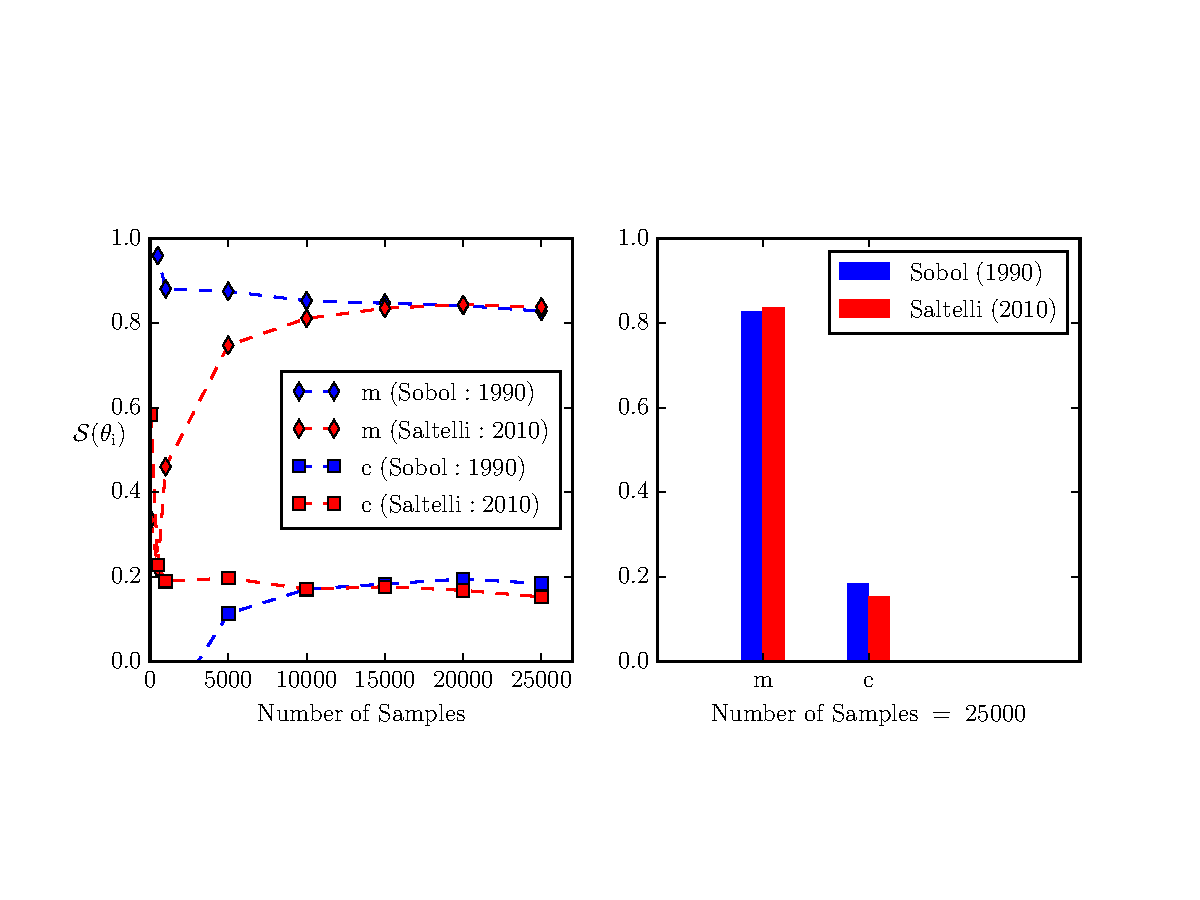
\includegraphics[width=1.0\textwidth]{./rawfigs/sensitivity_plot.pdf}
\end{center}
\caption{(a) Analysis of convergence for the first order sensitivity indices for slope, $m$ and
y-intercept, $c$ with increasing sample size. (b) Bar-graph representation of estimates for $\mathcal{S}(\theta_{i})$
based on estimators suggested by Sobol~\cite{Sobol:1990} and Saltelli~\emph{et al.}~\cite{Saltelli:2010} using 25000
pseudo-random samples.}
\label{fig:sensitivity}
\end{figure}

Figure~\ref{fig:sensitivity}(b), illustrates estimates for $\mathcal{S}(\theta_{i})$ for the slope, $m$ and the
y-intercept, $c$ based on 25000 samples. For both parameters, estimates from Sobol~\cite{Sobol:1990} and 
Saltelli~\emph{et al.}~\cite{Saltelli:2010} are in close agreement. Moreover, the QoI ($y$) is observed
to be much more sensitive to the uncertainty in the slope as compared to the y-intercept. 

\section{Concluding Remarks}

Global Sensitivity Analysis can be a computationally challenging task especially  if it involves model
estimates for a complex multiphysics problem. However, in case the forward solve of the model is inexpensive, one
can exploit the SFP machinery in QUESO to compute the sensitivity indices as demonstrated with the
help of a simple example in this chapter. Moreover, when stochastic formulations are proposed to
capture the inadequacy in a model, parametric sensitivity analysis based on prior distributions of
the stochastic parameters can potentially reduce the dimensionality of an inverse problem.
Depending upon the nature of the problem, one can benefit from valuable insight into relative
importance of the parameters with much fewer samples than required for convergence of the estimates as
observed in the case of the straight line problem discussed in this chapter.  
 



















